%
% ellipsenbogen.tex
%
% (c) 2021 Prof Dr Andreas Müller, OST Ostschweizer Fachhochschule
%
\section{Bogenlänge 
\label{buch:geometrie:section:ellipsenbogen}}
\rhead{Bogenlänge}
Die Möglichkeit, die Länge einer Kurve zu definieren und zu bestimmen,
ist eine der Leistungen der Infinitesimalrechnung.
In einigen Fällen lässt sich die Länge auch auf elementare Art und
Weise bestimmen oder mit Integralen, die leicht auflösbar sind.
Bereits bei der Bogenlänge entlang einer Ellipse sieht die Lage
jedoch ganz anders aus.

\subsection{Berechnung der Bogenlänge}
In diesem Abschnitt sollen ein paar Methoden zusammgengestellt werden,
mit denen die Länge einer Kurve berechnet werden kann.

\subsubsection{Länge einer parametrisierten Kurve}
Beispiele wie die Kochsche Schneeflockenkurve, deren Länge schwer
zu definieren ist, zeigen, dass der Begriff einer Kurve für die Zwecke
dieses Abschnittes genügend eng gefasst werden muss.
Die folgende Definition tut dies.

\begin{definition}
\label{buch:geometrie:def:kurve}
Sei $I=[a,b]\subset\mathbb{R}$ ein Intervall.
Eine {\em Kurve} ist eine differenzierbare Abbildung
$\gamma \colon I \to \mathbb{R}^n$.
\index{Kurve}
\end{definition}

\begin{beispiel}
\begin{figure}
\centering
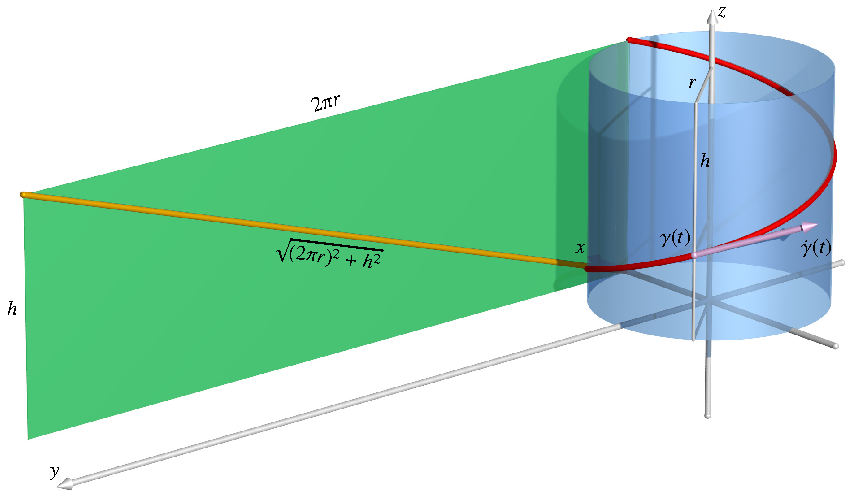
\includegraphics[width=\textwidth]{chapters/030-geometrie/images/zylinder.pdf}
\caption{Schraubenlinie mit der Parameterdarstellung
\eqref{buch:geometrie:eqn:helix} und Abrollung zur Berechnung der
Länge der Kurve.
\label{buch:geometrie:fig:zylinder}}
\end{figure}
Die Abbildung~\ref{buch:geometrie:fig:zylinder} zeigt 
\begin{equation}
\gamma
\colon
[0,2\pi] \to \mathbb{R}^3
:
t\mapsto\begin{pmatrix}r\cos t\\ r\sin t\\ th/2\pi\end{pmatrix}
\label{buch:geometrie:eqn:helix}
\end{equation}
beschreibt eine Schraubenlinie oder Helix.
\index{Schraubenlinie}%
\index{Helix}%
Die Abbildung ist ganz offensichtlich differenzierbar und hat die
Ableitung
\begin{equation}
\frac{d}{dt}\gamma(t)
=
\dot{\gamma}(t)
=
\begin{pmatrix} -r\sin t \\ r\cos t \\ h/2\pi\end{pmatrix}.
\label{buch:geometrie:eqn:helixdot}
\end{equation}
Die Länge dieser Schraubenlinie lässt sich direkt berechnen.
Die Schraubenlinie liegt auf dem Mantel eines Zylinders mit
Radius $r$ und Höhe $h$.
Durch Abrollen des Zylinders erkennt man, dass die Schraubenlinie
die Hypothenuse eines rechtwinkligen Dreiecks mit Katheten 
$2\pi r$ und $h$ ist.
Die Länge $l$ der Schraubenlinie ist daher
\begin{equation}
l = \sqrt{(2\pi r)^2 +h^2}
\label{buch:geometrie:eqn:helixlaenge}
\end{equation}
nach dem Satz von Pythagoras.
\end{beispiel}

Unterteilt man das Intervall $I$ in den Teilpunkten $t_i$ mit
\[
a = t_0 < t_1 < t_2 < \dots < t_{n-1} < t_n = b,
\]
dann ist die Summe
\[
L
=
\sum_{i=0}^{n-1} |\gamma(t_{i+1}) - \gamma(t_{i})|
\]
eine Approximation für die Länge der Kurve.
Die Differenz auffeinanderfolgender Punkte kann mit Hilfe der
Ableitung als
\[
\gamma(t_{i+1})-\gamma(t_i)
\approx
\dot{\gamma}(t_{i}) \cdot (t_{i+1}-t_i)
\]
approximiert werden.
Damit wird die Summe $L$ approximiert durch
\[
L\approx \sum_{i=0}^{n-1} |\dot{\gamma}(t_i)| \cdot (t_{i+1}-t_i).
\]
Dies ist eine Riemannsche Summe für das Integral
\[
\int_a^b |\dot{\gamma}(t)|\,dt,
\]
wir definieren die Bogenlänge einer Kurve daher wie folgt.

\begin{definition}
\label{buch:geometrie:def:kurvenlaenge}
Sei $\gamma\colon I\to\mathbb{R}$ eine Kurve im Sinne der
Definition~\ref{buch:geometrie:def:kurve}.
Dann ist die {\em Bogenlänge} entlang der Kurve zwischen dem Punkt
$\gamma(a)$ und $\gamma(t)$ definiert durch das
Integral
\[
l(t) = \int_{a}^t |\dot{\gamma}(\tau)|\,d\tau.
\]
\end{definition}

\begin{beispiel}
Die Helix mit der Parametrisierung~\eqref{buch:geometrie:eqn:helix}
hat die Kurvenlänge
\begin{align*}
l(t)
&=
\int_0^t |\dot{\gamma}(\tau)|\,d\tau
=
\int_0^t \sqrt{r^2\sin^2 \tau + r^2\cos^2\tau + (h/2\pi)^2}\,d\tau
\\
&=
\int_0^t \sqrt{r^2 + (h/2\pi)^2}\,d\tau
=
t\sqrt{r^2+(h/2\pi)^2}.
\end{align*}
Für eine ganze Umdrehung, also für $t=2\pi$ finden wir
\(
l(2\pi) = \sqrt{4\pi^2 r^2 + h^2},
\)
was mit dem elementaren Resultat~\eqref{buch:geometrie:eqn:helixlaenge}
übereinstimmt.
\end{beispiel}

\subsubsection{Länge eines Graphen}
Der Graph einer auf dem Intervall $I=[a,b]$ definierte Funktion
$y=f(x)$ kann als Parametrisierung einer Kurve
\[
\gamma
\colon
[a,b] \to \mathbb{R}^2
:
x \mapsto \begin{pmatrix}x\\f(x)\end{pmatrix}
\]
betrachtet werden.
Nach Definition~\ref{buch:geometrie:def:kurvenlaenge}
ist Länge dieser Kurven zwischen den Punkten $(a,f(a))$ und $(x,f(x))$
durch das Integral
\[
l(x)
=
\int_a^x \biggl| \begin{pmatrix}1\\f'(\xi)\end{pmatrix}\biggr|\,d\xi
=
\int_a^x \sqrt{1+f'(\xi)^2}\,d\xi
\]
gegeben.

\begin{beispiel}
Die auf dem Intervall $I=[0,b]$ definierte quadratische Funktion $f(x)=cx^2$
mit $b>0$ und $c>0$ hat die Bogenlänge
\begin{align*}
l(x)
&=
\int_0^x \sqrt{1+f'(\xi)^2}\,d\xi
=
\int_0^x \sqrt{1+4c^2\xi^2}\,d\xi
=
\biggl[
\frac{ \operatorname{arsinh}2c\xi)}{4c} + \frac{\xi\sqrt{4c^2\xi^2+1}}{2}
\biggr]_0^x
\\
&=
\frac{ \operatorname{arsinh}(2cx)}{4c}.
\end{align*}
Die Stammfunktion wurde mit einem Computeralgebraprogramm gefunden.
\end{beispiel}

\subsubsection{Kurvenlänge in Polarkoordinaten}
Eine Kurve kann in Polarkoordinaten in der Ebene durch eine Funktion
$r=r(\varphi)$ beschrieben werden.
Dies führt auf eine Parametrisierung
\[
\varphi \mapsto \gamma(\varphi)=\begin{pmatrix}
r(\varphi)\cos\varphi\\
r(\varphi)\sin\varphi
\end{pmatrix}
\]
durch den Polarwinkel $\varphi$.
Die Kurvenlänge kann gemäss 
Definition~\label{buch:geometrie:def:kurvenlaenge} braucht
die Ableitung der Parametrisierung, also die Funktion
\[
\dot{\gamma}(\varphi)
=
\begin{pmatrix}
r'(\varphi)\cos\varphi - r(\varphi)\sin\varphi\\
r'(\varphi)\sin\varphi + r(\varphi)\cos\varphi
\end{pmatrix}.
\]
Die Länge von $\dot{\gamma}$ ist
\begin{align*}
|\dot{\gamma}(\varphi)|^2
&=
\bigl(
r'(\varphi)\cos\varphi - r(\varphi)\sin\varphi
\bigr)^2
+
\bigl(
r'(\varphi)\sin\varphi + r(\varphi)\cos\varphi
\bigr)^2
\\
&=
r'(\varphi)^2\cos^2\varphi
-2r(\varphi)r'(\varphi)\cos\varphi\sin\varphi
+r(\varphi)^2\sin^2\varphi
\\
&\qquad
+r'(\varphi)^2\sin^2\varphi
+2r(\varphi)r'(\varphi)\sin\varphi\cos\varphi
+r(\varphi)^2\cos^2\varphi
\\
&=r'(\varphi)^2(\cos^2\varphi+\sin^2\varphi)
+ r(\varphi)^2(\sin^2\varphi+\cos^2\varphi)
\\
&=
r'(\varphi)^2 + r(\varphi)^2.
\end{align*}
Dies führt auf das
Integral
\begin{equation}
l(\alpha)
=
\int_a^\alpha \sqrt{r'(\varphi)^2 + r(\varphi)^2}\,d\varphi
\end{equation}
für die Länge der Kurve.

%
% hierhin verschoben für bessere Platzierung
%
\begin{figure}
\centering
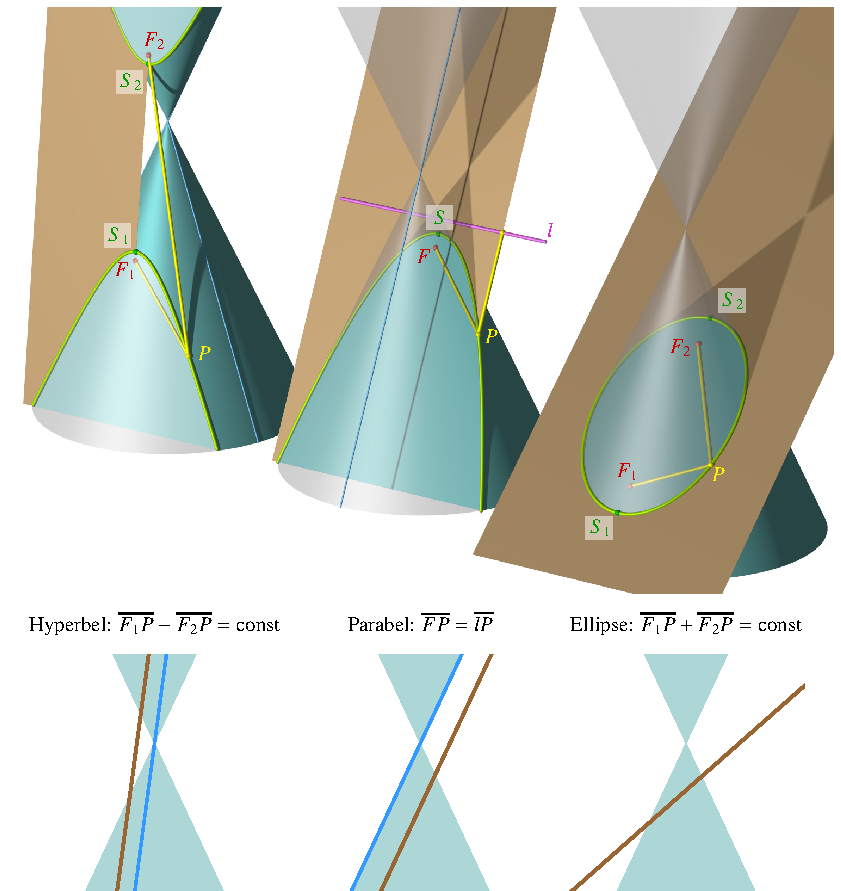
\includegraphics{chapters/030-geometrie/images/kegelschnitte.pdf}
\caption{Hyperbeln, Parabeln und Ellipsen sind die Schnittkurven einer
Ebene mit einem Kegel.
Der Winkel zwischen der Achse des Kegels und der Schnittebene bestimmt,
welche Art von Schnittkurve entsteht.
Wenn keine der Mantellinien des Kegels parallel ist zur Ebene, dann
entsteht eine Ellipse (rechts).
In der Mitte ist genau eine Mantellinie (hellblau) parallel zur Ebene,
es ensteht eine Parabel und links gibt es genau zwei verschiedene
Mantellinien des Kegels (hellblau), die zur Ebene parallel sind,
es entsteht eine Hyperbel.
\label{buch:geometrie:laenge:fig:kegelschnitte}}
\end{figure}
%

%
% Kreis
%
\subsection{Kreis}
Die Länge eines Bogens auf dem Einheitskreis zwischen dem Punkt
$(1,0)$ und $P=(x,y)$ mit $x^2+y^2=1$ ist nach Definition der
Winkel $\alpha$ zwischen der $x$-Achse und $P$.
Es gilt also
\[
\tan\alpha = \frac{y}{x}
\qquad\text{oder}\qquad
\sin\alpha = y = \sqrt{1-x^2}.
\]
Der Kreis kann auch als Graph $y=f(x)=\sqrt{1-x^2}$ parametrisiert werden,
in der die Länge des Bogens 
\begin{align*}
l(x)
=
\int_x^1 \sqrt{1+f'(t)^2}\,dt
=
\int_x^1 \sqrt{1+\frac{t^2}{1-t^2}}\,dt
=
\int_x^1 \sqrt{\frac{1-t^2+t^2}{1-t^2}}\,dt
=
\int_x^1 \frac{dt}{\sqrt{1-t^2}}.
\end{align*}
Aus dem bekannten Wert der Länge des Bogens erhalten wir jetzt die
Formel
\begin{equation}
\arcsin \sqrt{1-x^2} = \int_x^1 \frac{dt}{\sqrt{1-t^2}}.
\label{buch:geometrie:eqn:kreislaenge} 
\end{equation}
Tatsächlich ist die Ableitung davon
\[
\frac{d}{dx}\arcsin\sqrt{1-x^2}
=
-\frac{1}{\sqrt{1-x^2}},
\]
was mit der Integralformel~\ref{buch:geometrie:eqn:kreislaenge} 
übereinstimmt.

\subsection{Kegelschnitte
\label{buch:geometrie:subsection:kegelschnitte}}
Kegelschnitte sind die Schnittkurven eines geraden Kreiskegels
mit einer Ebene (Abbildung~\ref{buch:geometrie:laenge:fig:kegelschnitte}).
Der Kreis ist der Spezialfall des Schnittes mit einer horizontalen
Ebene.
Im Gegensatz zum Kreis lässt sich aber die Kurvenlänge nicht mehr
in geschlossener Form berechnen.

\subsubsection{Koordinatengleichung}
Aus der in Abbildung~\ref{buch:geometrie:laenge:fig:kegelschnitte}
dargestellten Geometrie kann man die folgende Charakterisierung von
Ellipsen und Hyperbeln ableiten.

\begin{definition}
\label{buch:geometrie:def:kegelschnitte}
Gegeben sind die Punkte $F_1$ und $F_2$ in der Ebene, sie heissen
die {\em Brennpunkte}.
Die Punkte in der Ebene, deren Abstandssumme von zwei festen Punkten $F_1$
und $F_2$ konstant ist, bilden eine {\em Ellipse}.
Die Punkte in der Ebene, deren Abstandsdifferenz von zwei festen Punkten
$F_1$ und $F_2$ konstant ist, bilden eine {\em Hyperbel}.
\end{definition}

\begin{figure}
\centering
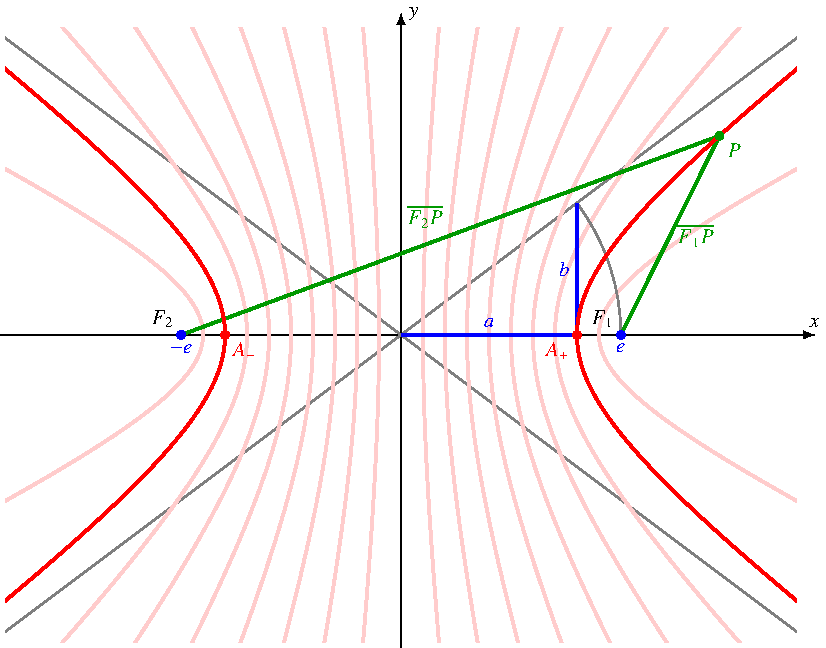
\includegraphics{chapters/030-geometrie/images/hyperbel.pdf}
\caption{Geometrie einer Hyperbel in der Ebene.
Die Hyperbel besteht aus den Punkten $P$ der Ebene, deren Entfernungsdifferenz
$\overline{F_1P}-\overline{F_2P}$
von zwei vorgegebenen Punkten $F_1$ und $F_2$ konstant ist.
Die Differenz $\pm 2a$ führt auf die Hyperbeln mit Halbachsen
$a$ und $b$.
\label{buch:geometrie:hyperbel:fig:2d}}
\end{figure}
\begin{figure}
\centering
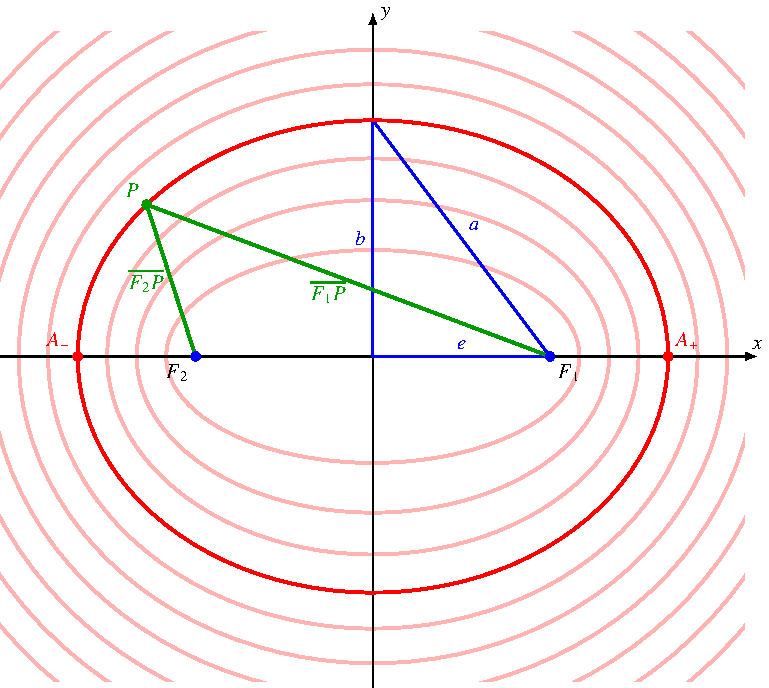
\includegraphics{chapters/030-geometrie/images/ellipse.pdf}
\caption{Geometrie einer Ellipse in der Ebene.
Die Ellipse besteht aus den Punkten $P$ der Ebene, deren Entfernungssumme
$\overline{F_1P}+\overline{F_2P}$
zu zwei vorgegebenen Punkten $F_1$ und $F_2$ konstant ist.
Die Summe $\pm 2a$ führt auf die Ellipsen mit Halbachsen
$a$ und $b$.
\label{buch:geometrie:ellipse:fig:2d}}
\end{figure}
Aus der Definition~\ref{buch:geometrie:def:kegelschnitte} soll jetzt
eine Koordinatengleichung für Ellipsen und Hyperbeln hergeleitet werden.
Die Brennpunkte haben die Koordinaten $F_1=(e,0)$ und $F_2=(-e,0)$.
Die Grösse $e$ heisst auch die {\em lineare Exzentrizität}.
Die Abstandssumme bzw.~-differenz wird mit $2a$ bezeichnet

Die Punkte $A_+=(a,0)$ und $A_-=(-a,0)$ sind Punkte der gesuchten
Kurven,
denn die Summe bzw.~Differenz der Entfernungen von $A_+$ zu den beiden
Brennpunkten ist
\[
\overline{A_+F_2}
\pm
\overline{A_+F_1}
=
\begin{cases}
(a-e)+(a+e) = 2a
&\qquad\text{Ellipse}
\\
(e+a)-(e-a) = 2a
&\qquad\text{Hyperbel}
\end{cases}
\]
In Abbildung~\ref{buch:geometrie:hyperbel:fig:2d} ist diese Situation
für eine Hyperbel dargestellt, in 
Abbildung~\ref{buch:geometrie:ellipse:fig:2d} für eine Ellipse.
Für eine Ellipse ist $e<a$, für eine Hyperbel ist $e>a$, wir schreiben
\[
b^2
=
\begin{cases}
a^2-e^2&\qquad\text{Ellipse} \\
e^2-a^2&\qquad\text{Hyperbel}
\end{cases}
\]
Die Zahlen $a$ und $b$ heissen die {\em grosse} bzw.~{\em kleine Halbachse}
der Ellipse bzw.~Hyperbel.

Für einen beliebigen Punkt $P=(x,y)$ in der Ebene wird die Bedingung
an die Abstände zu
\[
\overline{PF_2}
\pm
\overline{PF_1}
=
\sqrt{(x+e)^2+y^2}
\pm
\sqrt{(x-e)^2+y^2}
=
2a.
\]
Hier und in der folgenden Rechnung gilt das obere Zeichen jeweils
für die Ellipse, das untere für die Hyperbel.
Quadrieren ergibt
\begin{align*}
4a^2
&=
(x+e)^2+y^2
\pm
2\sqrt{
((x+e)^2+y^2)
((x-e)^2+y^2)
}
+
(x-e)^2+y^2
\\
2a^2-x^2-e^2-y^2
&=
\pm\sqrt{
y^4 + y^2((x+e)^2 + (x-e)^2) +(x^2-e^2)^2
}
\\
&=
\pm\sqrt{y^4 + 2y^2 ( x^2+e^2) +x^4 - 2x^2e^2 + e^4}.
\end{align*}
Erneutes Quadrieren bringt auch die Wurzel auf der rechten Seiten
zum Verschwinden:
\begin{align}
4a^4 + x^4 + e^4 + y^4
-4a^2(x^2+y^2+e^2)
+2y^2(x^2+e^2)+2x^2e^2
&=
y^4+2y^2(x^2 +e^2) + x^4 -2x^2e^2+e^4
\notag
\\
4a^4
-4a^2(x^2+y^2+e^2)
+2x^2e^2
&=
-2x^2e^2
\notag
\\
a^4+x^2e^2&=a^2(x^2+y^2+e^2)
\notag
\\
x^2(e^2-a^2)&=a^2(e^2-a^2) + a^2y^2.
\notag
\end{align}
Die Differenz $e^2-a^2$ ist bis auf das Vorzeichen identisch mit $b^2$,
genauer gilt
\begin{equation*}
\mp x^2b^2 = \mp a^2b^2 + a^2y^2.
\end{equation*}
Nach Division durch $\mp a^2b^2$ bleibt
\begin{equation}
\frac{x^2}{a^2} = 1 \mp{y^2}{b^2}
\qquad\Rightarrow\qquad
\frac{x^2}{a^2} \pm \frac{y^2}{b^2} = 1,
\label{buch:geometrie:hyperbel:gleichung}
\end{equation}
die Koordinatengleichunggleichung einer Ellipse bwz.~Hyperbel.


\subsubsection{Hyperbeln}
Die Hyperbeln können auch als Graphen einer Funktion von $x$ gefunden werden.
Dazu wird die Gleichung~\eqref{buch:geometrie:hyperbel:gleichung}
nach $y$ aufgelöst:
\[
\frac{x^2}{a^2}
-
\frac{y^2}{b^2}
=
1
\qquad\Rightarrow\qquad
y
=
\pm
b\sqrt{\frac{x^2}{a^2}-1}.
\]
Die rechte Seite hat für $|x|<a$ keine reellen Werte.
Ebenso kann die Hyperbel als Graph der Funktion
\[
y\mapsto x = \pm a\sqrt{1+\frac{y^2}{b^2}}
\]
dargestellt werden, die für alle $x\in\mathbb{R}$ definiert ist und
nur Werte mit Betrag $\ge a$ hat.

Ein besonders einfacher Spezialfall ist $a=b=1$, genannt eine
{\em gleichseitige Hyperbel}.
\index{gleichseitige Hyperbel}%
\index{Hyperbel, gleichseitig}%
In diesem Fall ist $x^2-y^2=1$ und $e^2=2$.

\subsubsection{Länge eines gleichseitigen Hyperbelbogens}
Die Funktion $f(x)=\sqrt{1+x^2}$ beschreibt eine gleichseitige
Hyperbel, die gegenüber der Situation in
Abbildung~\ref{buch:geometrie:hyperbel:fig:2d}
an der Winkelhalbierenden des ersten Quadranten gespiegelt ist.
Die Bogenlänge zwischen dem Punkt $(0,1)$ und $(x,y)$ auf der
Hyperbel ist gegeben durch das Integral:
\[
l(x)
=
\int_0^x \sqrt{1+f'(t)^2}\,dt
=
\int_0^x \sqrt{1+\frac{t^2}{1+t^2}}\,dt
=
\int_0^x \sqrt{\frac{1+2t^2}{1+t^2}}\,dt.
\]
Dieses Integral ist nicht in geschlossener Form lösbar.
Natürlich können auch andere Parametrisierungen für die Hyperbel
verwendet werden, die entstehenden Integrals, dies ändert jedoch
nichts an der Schwierigkeit, einen Ausdruck für den Wert des
Integrals anzugeben.

\subsubsection{Parametrisierung mit hyperbolischen Funktionen}
Etwas allgemeiner wird eine Hyperbel durch die Gleichung
\begin{equation}
\frac{x^2}{a^2} - \frac{y^2}{b^2} = 1
\label{buch:geometrie:hyperbel:eqn}
\end{equation}
beschrieben.
Die hyperbolischen Funktionen parametrisieren alle Paare von Zahlen
$(X,Y)=(\cosh t,\sinh t)$ mit der Eigenschaft $X^2-Y^2=1$.
Aus \eqref{buch:geometrie:hyperbel:eqn} folgt daher, dass
\[
\frac{x}{a} = \cosh t,\quad \frac{y}{b} = \sinh t
\qquad\Rightarrow\qquad
x=a\cosh t,\quad y=b\sinh t.
\]
Somit ist 
\[
\gamma\colon
\mathbb{R}\to\mathbb{R}^2
:
t\mapsto \begin{pmatrix}a\cosh t\\b\sinh t\end{pmatrix}
\]
eine Parametrisierung der Hyperbel.
Für die Länge eines Hyperbelbogens zwischen zwei Parameterwerten
$t_0$ und $t_1$ wird dann
\begin{align*}
l
&=
\int_{t_0}^{t_1}
\sqrt{a^2 \sinh^2 t + b^2 \cosh^2 t}
\,dt
=
\int_{t_0}^{t_1}
\sqrt{a^2 \sinh^2 t + b^2 (1+\sinh^2 t)}
\,dt
\\
&=
b
\int_{t_0}^{t_1}
\sqrt{1 + \frac{a^2+b^2}{b^2} \sinh^2 t }
\,dt
=
b
\int_{t_0}^{t_1}
\sqrt{1 + \frac{e^2}{b^2} \sinh^2 t }
\,dt.
\end{align*}
Das Integral auf der rechten Seite ist nicht mit elementaren Funktionen
ausführbar und rechtfertigt die Definition neuer spezieller Funktionen.
Die Kurvenlänge auf einer Hyperbel kann mit den in
Kapitel~\ref{buch:chapter:elliptischefunktionen}
beschriebenen elliptischen Integralen beschrieben werden.
\begin{figure}
\centering
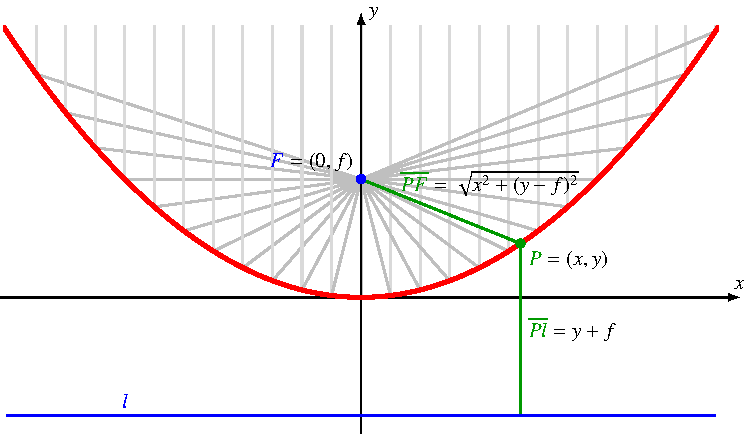
\includegraphics{chapters/030-geometrie/images/parabel.pdf}
\caption{Eine Parabel ist die Menge der Punkte, die von der Geraden $l$
und dem Brennpunkt $F$ gleichen Abstand haben.
\label{buch:geometrie:fig:parabel}}
\end{figure}

\subsubsection{Ellipsen}
Sei $(x,y)$ ein Punkt, der die
Ellipsengleichung~\eqref{buch:geometrie:hyperbel:gleichung} erfüllt.
Dann erfüllt $(X,Y)=(x/a, y/b)$ die Gleichung $X^2+Y^2=1$, ein Punkt auf
einem Kreis.
Insbesondere gibt es ein $t\in\mathbb{R}$ derart, dass
\[
\frac{x}{a} = \cos t ,\quad \frac{y}{b}=\sin t
\qquad\Rightarrow\qquad
x=a\cos t,\quad y=b\sin t.
\]
Somit ist
\[
\gamma
\colon
\mathbb{R}\to\mathbb{R}^2
:
t \mapsto\begin{pmatrix}a\cos t\\b\sin t\end{pmatrix}
\]
eine Parametrisierung der Ellipse.
Die Länge eines Ellipsenbogens zwischen den Winkelargumenten $\alpha$ und
$\beta$ ist dann
\begin{align*}
l(\alpha,\beta)
&=
\int_\alpha^\beta
\sqrt{
a^2 \sin^2 t + b^2 \cos^2t
}
\,dt
=
\int_\alpha^\beta
\sqrt{
a^2 - (a^2-b^2)\cos^2 t
}
\,dt
\\
&=
a
\int_\alpha^\beta
\sqrt{
1 - \frac{a^2-b^2}{a^2} \cos^2t
}
\,dt
=
a\int_\alpha^\beta
\sqrt{
1-\varepsilon^2 \cos^2t
}
\,dt.
\end{align*}
Auch dieses Integral ist nicht in geschlossener Form lösbar.
Dies motiviert in Kapitel~\ref{buch:chapter:elliptischefunktionen}
die Definition~\ref{buch:elliptisch:def:integrale123}
der sogenannten elliptischen Integrale als neue
spezielle Funktionen.
Auf Seite~\pageref{buch:elliptisch:fig:ellipsenumfang} wird gezeigt,
dass der Umfang einer Ellipse $4aE(\varepsilon)$ ist,
wobei $\varepsilon=e/a$ und $e^2=a^2-b^2$ (siehe auch
Abbildung~\ref{buch:elliptisch:fig:ellipsenumfang}).

\subsubsection{Parabeln}
Aus der Geometrie der Kegelschnitte
(Abbildung~\ref{buch:geometrie:def:kegelschnitte})
kann auch die folgende Charakterisierung einer Parabel abgeleitet werden.

\begin{definition}
\label{buch:geometrie:def:parabel}
Sei $F$ ein Punkt in der Ebene $l$ eine Gerade, die $F$ nicht enthält.
$F$ heisst {\em Brennpunkt}, $l$ heisst {\em Leitgerade} der Parabel.
Die Menge aller Punkte $P$, die von $F$ und $l$ den gleichen
Abstand haben, heisst {\em Parabel}.
Die {\em Brennweite} $f$ ist der halbe Abstand von $F$ zu $l$,
also $\overline{Fl}=2f$.
\end{definition}

Ohne Einschränkung der Allgemeinheit kann man $F=(0,f)$ und
$l$ als die Gerade $y=-f$ annehmen
(siehe Abbildung~\ref{buch:geometrie:fig:parabel}).
Ein Punkt $P=(x,y)$ liegt genau dann auf der Parabel, wenn
\begin{align*}
\overline{Pl}
&=
\overline{PF}
\\
(y+f)^2
&=
x^2 + (y-f)^2
\\
y^2+2yf+f^2
&=
x^2 + y^2-2yf+f^2
\\
4yf
&=
x^2
\qquad\Rightarrow\qquad y=\frac{1}{4f}x^2.
\end{align*}
Eine Parabel ist also der Graph einer quadratischen Funktion.

Parabeln haben erhebliche praktische Bedeutung, weil sie parallel zur
Achse einfallende Strahlen im Brennpunkt $F$ fokusieren.

\subsubsection{Bogenlänge einer Parabel}
Die Länge eines Parabelbogens zwischen $x_1$ und $x_2$ ist
\begin{align*}
l(x_1,x_2)
&=
\int_{x_1}^{x_2}
\sqrt{1+\biggl(\frac{1}{2f}x\biggr)^2}
\,dx
\end{align*}
Mit der Substitution $x=2ft$ wird das Integral zu
\[
l(x_1,x_2)
=
2f
\int_{x_1/2f}^{x_2/2f}
\sqrt{1+t^2}
\,dt
=
f\biggl[
\operatorname{arsinh} t +t\sqrt{1+t^2}
\biggr]_{x_1/2f}^{x_2/2f}
=
\biggl[
f
\operatorname{arsinh}\frac{x}{2f}
+
\frac{x}{4f}\sqrt{4f^2+x^2}
\biggr]_{x_1}^{x_2}.
\]
Während also Ellipsen- und Hyperbelbogen nicht in geschlossener
Form berechnet werden können, ist dies für Parabelbögen sehr wohl
möglich.




